\documentclass{beamer}
\usepackage{tikz}
\usepackage{verbatim}
\usetheme{Warsaw}
\title{Intersection Management with Constraint-Based Reservation
System}
\author{Tsz-Chiu Au, Shun Zhang, Peter Stone\\ Department of Computer
Science\\ The University of Texas at Austin}

\defbeamertemplate*{footline}{shadow theme}
{%
  \leavevmode%
  \hbox{\begin{beamercolorbox}[wd=.5\paperwidth,ht=2.5ex,dp=1.125ex,leftskip=.3cm plus1fil,rightskip=.3cm]{author in head/foot}%
    \usebeamerfont{author in head/foot}\insertframenumber\,/\,\inserttotalframenumber\hfill\insertshortauthor
  \end{beamercolorbox}%
  \begin{beamercolorbox}[wd=.5\paperwidth,ht=2.5ex,dp=1.125ex,leftskip=.3cm,rightskip=.3cm plus1fil]{title in head/foot}%
    \usebeamerfont{title in head/foot}\insertshorttitle%
  \end{beamercolorbox}}%
}

\begin{document}

\begin{frame}
\titlepage
\end{frame}

\section{Introduction}

\subsection{Autonomous Intersection Management}

\begin{frame}{Transportation Infrastructure: Present and Future}
\begin{columns}[c]
	\column{.6\textwidth}
		\begin{itemize}
		\item Today’s transportation infrastructure is designed for
		human drivers.\pause
		\item In the future: \textbf{Autonomous Intersection
		Management}\\
		Utilize the capacity of autonomous vehicles to improve traffic
		in transportation systems.
		\end{itemize}
		
	\column{.4\textwidth}
		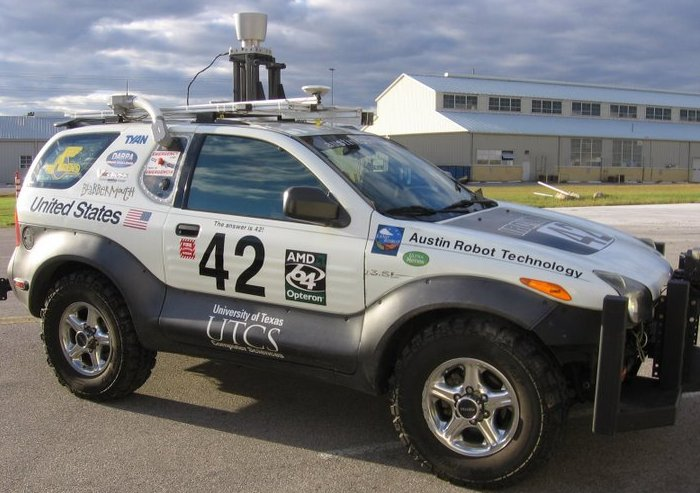
\includegraphics[width=0.8\textwidth]{42.png}
		\hfill
		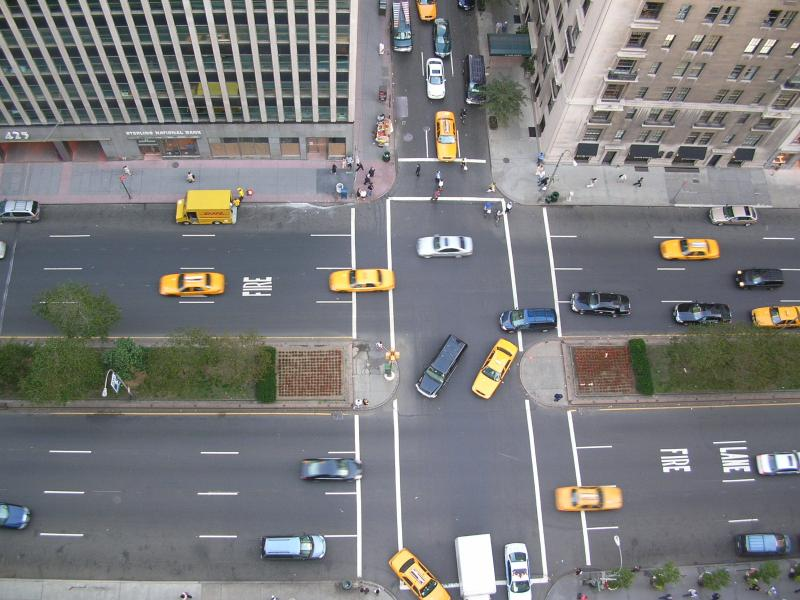
\includegraphics[width=0.8\textwidth]{intersection.jpg}
\end{columns}
\end{frame}

\begin{frame}{Autonomous Intersection Management}
\begin{columns}[c]
	\column{.4\textwidth}
		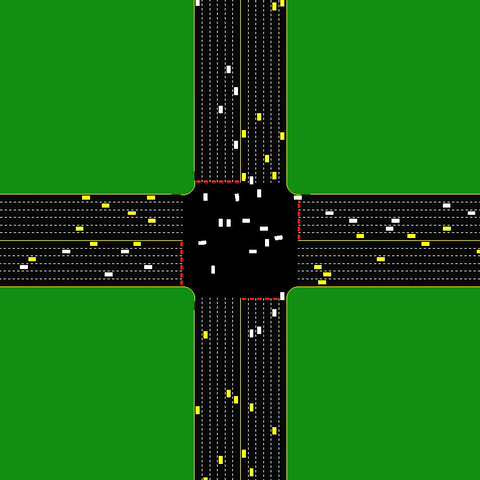
\includegraphics[width=\textwidth]{aim.png}
				
	\column{.6\textwidth}
		\begin{itemize}
		\item Dramatically reduce the traffic delay.
		\item Reduce the overhead of fuel consumption by approximately
		two thirds. \cite{bib:Dresner08Multiagent}
		\end{itemize}
\end{columns}
\end{frame}

\begin{frame}{Grid-Based Collision Detection}
	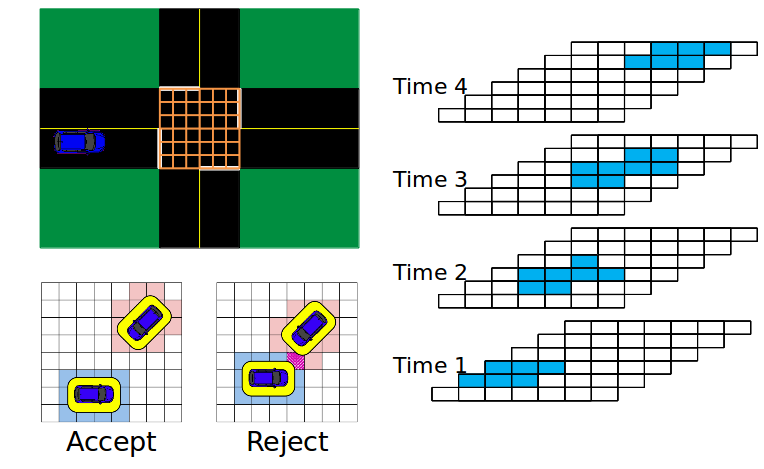
\includegraphics[width=\textwidth]{grids.png}
\end{frame}

\section{Semi-Autonomous Intersection Manangement}

\subsection{Motivation}

\begin{frame}{Sharing the Road with Human Drivers}
\begin{columns}[c]
\column{.6\textwidth}
\begin{itemize}
\item AIM is designed for the time when vehicles are autonomous.
\item Autonomous vehicles won't displace manual-controlled vehicles in one
day. Some people enjoy driving.\pause
\item One solution: FCFS-light = First-Come First-Served Policy + Traffic Signals
\end{itemize}
\column{.4\textwidth}
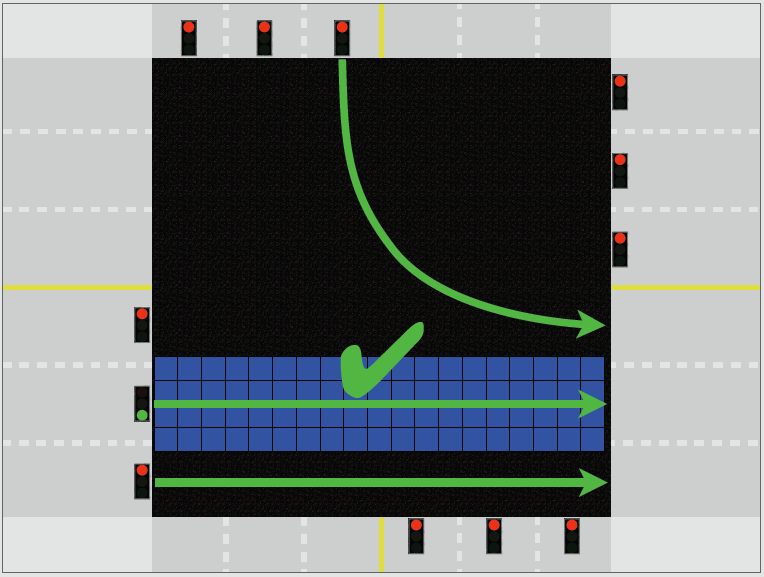
\includegraphics[width=\textwidth]{fcfs-light-1.png}
\hfill
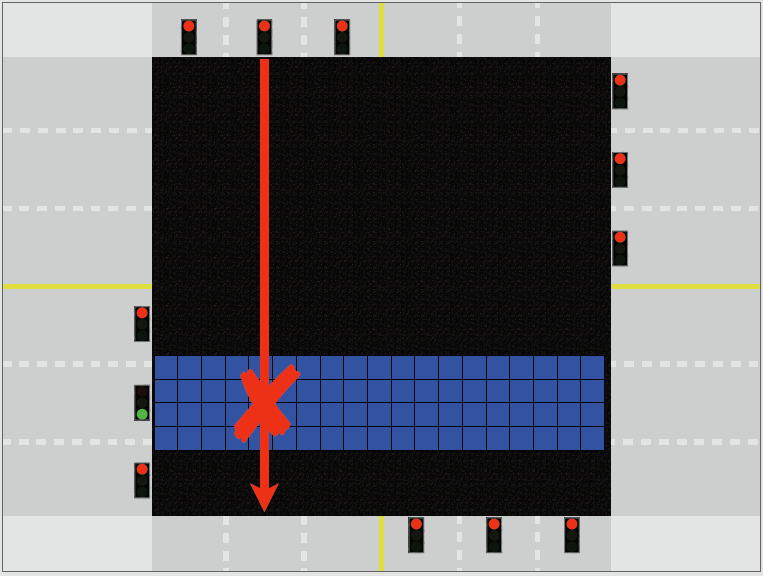
\includegraphics[width=\textwidth]{fcfs-light-2.png}
\end{columns}
\end{frame}

\begin{frame}{Observation}
\begin{itemize}
\item This ignores the possible equipments of human-driven vehicles
(e.g.\ cruise control).\pause
\item \textbf{Goal}: find a way to make all types of vehicles to
achieve the benefits (better than traffic signal, may not be as good
as fully autonomous vehicles).
\end{itemize}
\end{frame}

\subsection{Semi-Autonomous Vechiles}

\begin{frame}{Definition}
\textbf{Semi-autonomous vehicles}: vehicles with limited autonomous
driving and wireless communication capabilities.\pause

\hfill

They are able to follow a \textit{limited number} of predictable
trajectories at intersections more precisely than human drivers.
\end{frame}

\begin{frame}{Set of Equipments}
\begin{itemize}
\item \textbf{Communication Device (Com)}:
a component in a vehicle's on-board electronic system that enables the
vehicle to wirelessly communicate with the transportation
infrastructure including the IM.\pause
\item \textbf{Simple Cruise Control (CC)}:
An optional speed control subsystem in vehicles' drivetrain that
automatically controls the vehicle speed by taking over the throttle
of the vehicles.\pause
\item \textbf{Adaptive Cruise Control (ACC)}:
an advanced cruise control system that automatically adjusts the speed
of a vehicle in order to maintain a certain distance from vehicles
ahead.
\end{itemize}
\end{frame}

\begin{frame}{Type of Semi-Autonomous Vehicles}
\begin{tabular}{|c|c|c|c|}
  \hline
  Vehicle Type & Communication & Cruise & Adaptive \\
               & Device & Control & Cruise Control \\
  \hline
  SA-ACC & X & X & X  \\
  \hline
  SA-CC & X & X &  \\
  \hline
  SA-Com & X & &  \\
  \hline
\end{tabular}
\end{frame}

\subsection{Interaction Model}

\begin{frame}{Interaction Model}
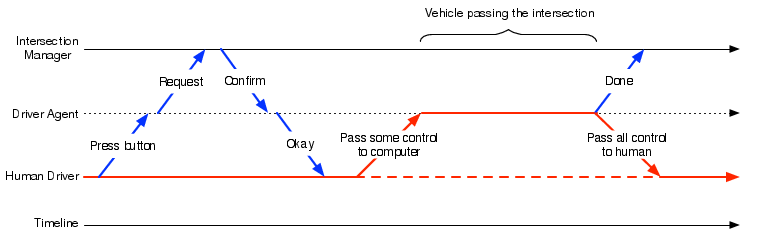
\includegraphics[width=\textwidth]{figures/interaction}
\end{frame}

\subsection{Constraint-Based Reservation Systems}

\begin{frame}{Constraint-Based Reservation}
We turn AIM into a \emph{constraint-based reservation system}, which
allows vehicles to make reservations in terms of constraints over
\begin{itemize}
\item their driving profiles such as their arrival time and arrival velocity
\item the relationships with other vehicles.
\end{itemize}
\end{frame}

\begin{frame}{Basic Elements}
\begin{itemize}
\item{\bf Intention}: The direction in which the vehicle intends to
move.\pause
\item{\bf Vehicle Type}: The type of vehicle.\pause
\item{\bf Entry Condition}: The condition under which the vehicle will
enter the intersection.\pause
\item{\bf Acceleration Profile List}: The list of possible
acceleration schedules from among which the vehicle will choose one to
follow during the traversal of the intersection.\pause
\end{itemize}
\end{frame}

\begin{frame}{Constant-Velocity Request}
\begin{itemize}
\item ${\sf Intent} = ( l_1 \vee l_2 \vee \ldots \vee l_n )$
in which $l_i$ is a possible lane from which the vehicle 
exits the intersection;
\item ${\sf Type}$ is the vehicle type;
\item ${\sf Entry} = (( l'_1 \vee l'_2 \vee \ldots \vee l'_n ), [t_1,\ t_2], [v_1,\ v_2])$
is the entry statement; and
\item ${\sf AP} = ( \langle (t_1, 0) \rangle )$
\end{itemize}

This is particularly used by Simple Cruise Control.
\end{frame}

\begin{frame}{Whole-Row Request}
\begin{itemize}
\item ${\sf Intent} = ( l_1 \vee l_2 \vee \ldots \vee l_n )$ $l_i$ is a possible lane from which the vehicle exits the intersection;
\item ${\sf Type}$ is the vehicle type;
\item ${\sf Entry} = (( l'_1 \vee l'_2 \vee \ldots \vee l'_n ), [t_1,\ t_2], [v_1,\ v_2])$ is the entry statement; and
\item ${\sf AP}$ is the acceleration profile list.
\end{itemize}

This is particularly used by Communication Device.
\end{frame}

\begin{frame}[fragile]{An General Request}
In Lisp syntax,

\begin{small}
\begin{verbatim}
(cc-profile (v verror angle)
  (is-auto-speed-control)
  (not is-auto-steering)
  (< velocity (+ v verror))
  (> velocity (- v verror))
  (< steer-angle angle) (> steer-angle -angle))
\end{verbatim}
\end{small}
\end{frame}

\section{Evaluations}

\begin{frame}{Evaluation on AIM}
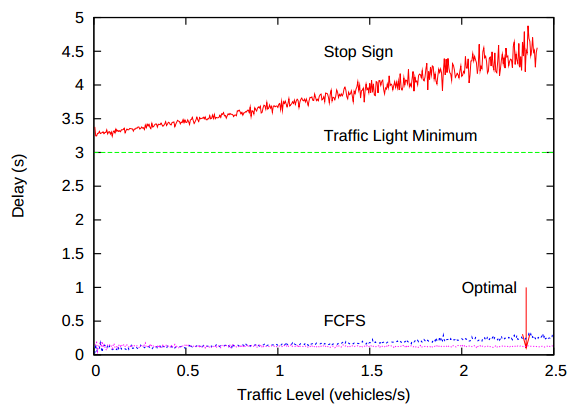
\includegraphics[width=0.8\textwidth]{old_result.png}
\end{frame}

\begin{frame}{Evaluation on SemiAIM}
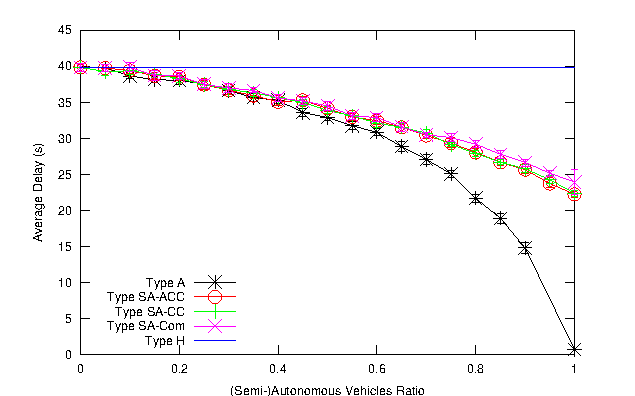
\includegraphics[width=0.9\textwidth]{figures/figure_1.pdf}

(Semi-)Autonomous vehicles vs. Human-Driven vehicles. Traffic
level = 360 vehicles/lane/hour.
\end{frame}

\begin{frame}{Evaluation on SemiAIM}
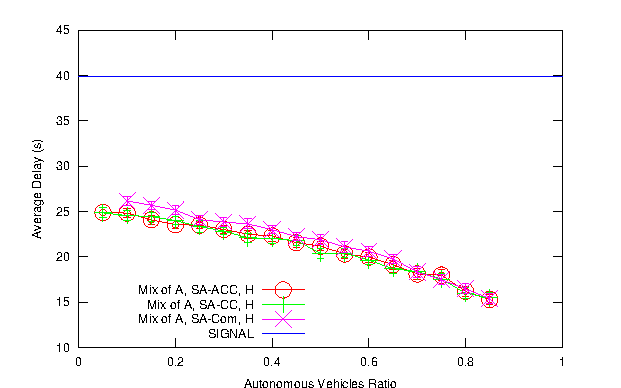
\includegraphics[width=0.9\columnwidth]{figures/figure_3.pdf}

The average delay according to a deployment schedule. Traffic level =
360 vehicles/lane/hour.
\end{frame}

\section{Conclusion}

\begin{frame}{Related Works}
\begin{itemize}
\item The main context of our work is an extension to the FCFS policy
proposed by Dresner and Stone \cite{bib:Dresner08Multiagent}.
\item Similar to the analysis of adaptive cruise control performance
by Jerath and Brennan \cite{bib:Jerath10adaptive}.
\item Part of a series of robotic car competitions such as the
\emph{DARPA Grand Challenges}~\cite{DARPAGrandChallenge}.
\item Autonomous vehicles can even outperform many human drivers in
carrying out intricate maneuvers~\cite{Squatriglia2010}.
\item etc.
\end{itemize}
\end{frame}

\begin{frame}{Conclusion}
\begin{itemize}
\item SemiAIM is the first multiagent protocol to enable smooth interactions
between human-driven, fully autonomous, and semiautonomous
vehicles.\pause
\item Our initial experiment showed that our system can greatly decrease
traffic delay when most vehicles are semiautonomous, even when few
(if any) are fully autonomous.
\end{itemize}
\end{frame}

\begin{frame}{Bibliography}
\tiny{\bibliographystyle{apalike}
\bibliography{bib/ref,bib/chiu,bib/intelligent_vehicles,bib/intersection,bib/peter}}
\end{frame}

\end{document}
